% Options for packages loaded elsewhere
\PassOptionsToPackage{unicode}{hyperref}
\PassOptionsToPackage{hyphens}{url}
\PassOptionsToPackage{dvipsnames,svgnames,x11names}{xcolor}
%
\documentclass[
  11pt,
]{article}

\usepackage{amsmath,amssymb}
\usepackage{iftex}
\ifPDFTeX
  \usepackage[T1]{fontenc}
  \usepackage[utf8]{inputenc}
  \usepackage{textcomp} % provide euro and other symbols
\else % if luatex or xetex
  \usepackage{unicode-math}
  \defaultfontfeatures{Scale=MatchLowercase}
  \defaultfontfeatures[\rmfamily]{Ligatures=TeX,Scale=1}
\fi
\usepackage{lmodern}
\ifPDFTeX\else  
    % xetex/luatex font selection
\fi
% Use upquote if available, for straight quotes in verbatim environments
\IfFileExists{upquote.sty}{\usepackage{upquote}}{}
\IfFileExists{microtype.sty}{% use microtype if available
  \usepackage[]{microtype}
  \UseMicrotypeSet[protrusion]{basicmath} % disable protrusion for tt fonts
}{}
\makeatletter
\@ifundefined{KOMAClassName}{% if non-KOMA class
  \IfFileExists{parskip.sty}{%
    \usepackage{parskip}
  }{% else
    \setlength{\parindent}{0pt}
    \setlength{\parskip}{6pt plus 2pt minus 1pt}}
}{% if KOMA class
  \KOMAoptions{parskip=half}}
\makeatother
\usepackage{xcolor}
\usepackage[left=2.54cm,right=2.54cm]{geometry}
\setlength{\emergencystretch}{3em} % prevent overfull lines
\setcounter{secnumdepth}{5}
% Make \paragraph and \subparagraph free-standing
\ifx\paragraph\undefined\else
  \let\oldparagraph\paragraph
  \renewcommand{\paragraph}[1]{\oldparagraph{#1}\mbox{}}
\fi
\ifx\subparagraph\undefined\else
  \let\oldsubparagraph\subparagraph
  \renewcommand{\subparagraph}[1]{\oldsubparagraph{#1}\mbox{}}
\fi


\providecommand{\tightlist}{%
  \setlength{\itemsep}{0pt}\setlength{\parskip}{0pt}}\usepackage{longtable,booktabs,array}
\usepackage{calc} % for calculating minipage widths
% Correct order of tables after \paragraph or \subparagraph
\usepackage{etoolbox}
\makeatletter
\patchcmd\longtable{\par}{\if@noskipsec\mbox{}\fi\par}{}{}
\makeatother
% Allow footnotes in longtable head/foot
\IfFileExists{footnotehyper.sty}{\usepackage{footnotehyper}}{\usepackage{footnote}}
\makesavenoteenv{longtable}
\usepackage{graphicx}
\makeatletter
\def\maxwidth{\ifdim\Gin@nat@width>\linewidth\linewidth\else\Gin@nat@width\fi}
\def\maxheight{\ifdim\Gin@nat@height>\textheight\textheight\else\Gin@nat@height\fi}
\makeatother
% Scale images if necessary, so that they will not overflow the page
% margins by default, and it is still possible to overwrite the defaults
% using explicit options in \includegraphics[width, height, ...]{}
\setkeys{Gin}{width=\maxwidth,height=\maxheight,keepaspectratio}
% Set default figure placement to htbp
\makeatletter
\def\fps@figure{htbp}
\makeatother
% definitions for citeproc citations
\NewDocumentCommand\citeproctext{}{}
\NewDocumentCommand\citeproc{mm}{%
  \begingroup\def\citeproctext{#2}\cite{#1}\endgroup}
\makeatletter
 % allow citations to break across lines
 \let\@cite@ofmt\@firstofone
 % avoid brackets around text for \cite:
 \def\@biblabel#1{}
 \def\@cite#1#2{{#1\if@tempswa , #2\fi}}
\makeatother
\newlength{\cslhangindent}
\setlength{\cslhangindent}{1.5em}
\newlength{\csllabelwidth}
\setlength{\csllabelwidth}{3em}
\newenvironment{CSLReferences}[2] % #1 hanging-indent, #2 entry-spacing
 {\begin{list}{}{%
  \setlength{\itemindent}{0pt}
  \setlength{\leftmargin}{0pt}
  \setlength{\parsep}{0pt}
  % turn on hanging indent if param 1 is 1
  \ifodd #1
   \setlength{\leftmargin}{\cslhangindent}
   \setlength{\itemindent}{-1\cslhangindent}
  \fi
  % set entry spacing
  \setlength{\itemsep}{#2\baselineskip}}}
 {\end{list}}
\usepackage{calc}
\newcommand{\CSLBlock}[1]{\hfill\break\parbox[t]{\linewidth}{\strut\ignorespaces#1\strut}}
\newcommand{\CSLLeftMargin}[1]{\parbox[t]{\csllabelwidth}{\strut#1\strut}}
\newcommand{\CSLRightInline}[1]{\parbox[t]{\linewidth - \csllabelwidth}{\strut#1\strut}}
\newcommand{\CSLIndent}[1]{\hspace{\cslhangindent}#1}

\usepackage[noblocks]{authblk}
\renewcommand*{\Authsep}{, }
\renewcommand*{\Authand}{, }
\renewcommand*{\Authands}{, }
\renewcommand\Affilfont{\small}
\usepackage{lipsum} \usepackage{libertine}
\makeatletter
\@ifpackageloaded{caption}{}{\usepackage{caption}}
\AtBeginDocument{%
\ifdefined\contentsname
  \renewcommand*\contentsname{Table of contents}
\else
  \newcommand\contentsname{Table of contents}
\fi
\ifdefined\listfigurename
  \renewcommand*\listfigurename{List of Figures}
\else
  \newcommand\listfigurename{List of Figures}
\fi
\ifdefined\listtablename
  \renewcommand*\listtablename{List of Tables}
\else
  \newcommand\listtablename{List of Tables}
\fi
\ifdefined\figurename
  \renewcommand*\figurename{Figure}
\else
  \newcommand\figurename{Figure}
\fi
\ifdefined\tablename
  \renewcommand*\tablename{Table}
\else
  \newcommand\tablename{Table}
\fi
}
\@ifpackageloaded{float}{}{\usepackage{float}}
\floatstyle{ruled}
\@ifundefined{c@chapter}{\newfloat{codelisting}{h}{lop}}{\newfloat{codelisting}{h}{lop}[chapter]}
\floatname{codelisting}{Listing}
\newcommand*\listoflistings{\listof{codelisting}{List of Listings}}
\makeatother
\makeatletter
\makeatother
\makeatletter
\@ifpackageloaded{caption}{}{\usepackage{caption}}
\@ifpackageloaded{subcaption}{}{\usepackage{subcaption}}
\makeatother
\ifLuaTeX
  \usepackage{selnolig}  % disable illegal ligatures
\fi
\usepackage{bookmark}

\IfFileExists{xurl.sty}{\usepackage{xurl}}{} % add URL line breaks if available
\urlstyle{same} % disable monospaced font for URLs
\hypersetup{
  pdftitle={Urban mobility and socioeconomic deprivation in Latin America after COVID-19},
  pdfauthor={Carmen Cabrera-Arnau; Francisco Rowe; Miguel González-Leonardo; Andrea Nasuto; Ruth Neville},
  colorlinks=true,
  linkcolor={blue},
  filecolor={Maroon},
  citecolor={Blue},
  urlcolor={Blue},
  pdfcreator={LaTeX via pandoc}}

\title{\textbf{Urban mobility and socioeconomic deprivation in Latin
America after COVID-19}}


\author[1]{Carmen Cabrera-Arnau}
\author[1]{Francisco Rowe}
\author[2]{Miguel González-Leonardo}
\author[1]{Andrea Nasuto}
\author[1]{Ruth Neville}

\affil[1]{Geographic Data Science Lab, Department of Geography and
Planning, University of Liverpool, Liverpool, UK}
\affil[2]{Centre for Demographic Urban and Environmental Studies, El
Colegio de México, Ciudad de México, México}


\date{}
\begin{document}
\maketitle
\begin{abstract}
The movement of people between locations is crucial for sustainable and
inclusive cities, facilitating the exchange of knowledge and resources.
Due to restrictions, lockdowns and fear of crowded places, the COVID-19
pandemic significantly reduced the number and extent of people's
movements. Existing research suggests that the impact of the pandemic on
mobility was unequal across locations and socioeconomic groups. However,
evidence and analysis of long-term changes in mobility is scarce,
especially in less developed countries. In this study, we use location
data from Meta-Facebook users to analyse patterns of urban mobility in X
Functional Urban Areas from South American countries. Findings reveal a
general decrease in mobility during the pandemic, with gradual recovery
trends up to April 2023. However, socioeconomic disparities are present
through the period of analysis, with deprived areas experiencing smaller
initial losses in mobility. These disparities generally diminish over
time, although they persist in all the countries included in the
analysis . Our research highlights the importance of timely mobility
data with high spatiotemporal resolution to understand the long-term
effects of the pandemic and inform equitable policy responses that
address societal challenges in urban areas.
\end{abstract}

\hfill\break

\section{Introduction}\label{sec-intro}

Spatial human mobility is key to creating sustainable, livable and
inclusive cities. At the societal level, spatial mobility enables the
transfer of knowledge, skills and labour to places they are
needed\textsuperscript{1}. Spatial mobility also shapes service and
transport demand across urban spaces\textsuperscript{2}, and enables the
monitoring and control of transmissible diseases\textsuperscript{3}. At
the individual level, mobility enables people to access and achieve
opportunities and aspirations in space\textsuperscript{4}. Understanding
spatial human mobility is thus important to supporting appropriate
policy responses to address societal challenges relating to carbon
emissions, urban planning, service delivery, public health, disaster
management and transport\textsuperscript{5,6}.

The COVID-19 pandemic resulted in a notable decrease in mobility,
particularly in cities\textsuperscript{7}. Coupled with fears of
contagion in crowded public spaces, nonpharmaceutical interventions to
contain the spread of COVID‐19 prompted this decrease in the overall
levels of mobility\textsuperscript{7,8}. Especially during lockdowns,
mobility recorded reductions in the frequency, distance and time of
trips in cities across the globe\textsuperscript{9--12}. Higher
engagement with remote working, online schooling and shopping activity
reduced the need to travel for work, education, shopping and leisure,
hence giving rise to more geographically localised mobility
patterns\textsuperscript{13}.

However, reductions in mobility levels were highly unequal reflecting
existing socioeconomic inequalities in our
societies\textsuperscript{14}. In most countries, affluent individuals
tended to record the greatest drops in mobility levels as they are
predominantly employed in knowledge-intensive jobs which can be done
fully or partly remotely\textsuperscript{10,15--18}. During the COVID-19
pandemic, the adoption of remote work reduced the need of commuting for
knowledge-intensive, non-public facing jobs\textsuperscript{19}. At the
same time, individuals from less privileged socioeconomic backgrounds
displayed less pronounced declines mirroring the nature of their work
requiring public-facing, face-to-face interaction, and thus a
requirement for daily work commutes\textsuperscript{17,18}.

Thus, while a growing body of empirical evidence has contributed to
advancing our understanding of the impacts of the COVID-19 pandemic on
spatial mobility within cities, existing research has focused on more
developed countries and the immediate effects of the pandemic during
2020. Less is known about the longer term patterns of resilience in
urban mobility in less developed countries extending beyond this
period\textsuperscript{20}. Urban spaces have changed considerably since
then, from going through waves of high COVID-19 fatality, infections,
school and business closures to the removal of all COVID-19 restrictions
as the UN World Health Organization (WHO) declared an end to the
pandemic as a public health emergency; yet, different configurations of
hybrid working have remained in the norm across many sector of the
economy\textsuperscript{21,22}. Thus, assessing the extent to which the
level of mobility has returned back to the pre-pandemic baseline level
across socioeconomic groups is important to understand the potentially
unequal long-term impacts of hybrid working.

A key barrier to monitor changes in geographic mobility patterns in less
developed countries during and post the COVID-19 pandemic has been the
lack of suitable data\textsuperscript{20}. Traditionally census and
survey data have been employed to analyse human mobility patterns in
these countries\textsuperscript{23}. Yet, these data streams are not
frequently updated and suffer from slow releases, with census data for
example being collected over intervals of ten years in most
countries\textsuperscript{24}. Traditional data streams thus lack the
temporal granularity to analyse population movements over short-time
periods and to offer an up-to-date representation of the urban mobility
system\textsuperscript{25}. Data resulting from social interactions on
digital platforms have emerged as an unique source of information to
deliver this representation and capture human population movement in
less developed countries at scale\textsuperscript{25}. Particularly
location data from mobile phone applications have become a prominent
source to sense patterns of human mobility at higher geographical and
temporal resolution in real time\textsuperscript{26}.

Drawing on a dataset of 213 million observations from Meta-Facebook
users' mobile location data, we aim to assess socioeconomic differences
in the extent and persistence of decline in urban mobility in Argentina,
Chile, Colombia and Mexico during and after the COVID-19 pandemic from
March 2020 to March 2023. We use Meta-Facebook data to measure
origin-destination flows from March 2020 to May 2022, and Meta Prophet
time-series forecasting machine learning algorithm\textsuperscript{27}
to predict origin-destination flows from June 2022 to March 2023. We use
Functional Urban Areas (FUAs) boundaries from the Global Human
Settlement Layer (GHSL), developed by the European Comission's Joint
Research Centre\textsuperscript{28} to define urban areas; and the
Global Gridded Relative Deprivation Index (GRDI) developed by NASA's
Socioeconomic Data and Applications Centre\textsuperscript{29} from
sociodemographic and satellite data inputs. Building on existing
evidence\textsuperscript{e.g. 30,31}, we hypothesised that (1) urban
mobility has recovered returning to the pre-pandemic baseline level of
movement as nonpharmaceuthical restrictions were lifted; and, that (2)
socioeconomic differences in urban mobility have endured the pandemic
reflecting deep societal inequalities as knowledge-intensive businesses
adopt hybrid working. \\

Latin America provides an ideal test-bed for testing these hypotheses
because of its exceptionally high levels of
inequalities\textsuperscript{32,33} and
urbanisation\textsuperscript{34}. Half of the 20 most unequal countries
in the planet are in this region. The average income Gini index of the
region is 4 percentage points higher than that of Africa and 11 higher
than China\textsuperscript{35}, and cities display some of the starkest
inequalities\textsuperscript{36}. Currently, over 80\% of the population
in Latin America live in urban areas. By 2050, this share is predicted
to reach 89\%, with the largest share concentrating in a few
megacities\textsuperscript{36}. Developing an understanding of human
mobility in Latin America is thus important to support sustainable and
inclusive spaces\textsuperscript{36}.

\section{Results}\label{sec-results}

The evolution of the percentage change in the number of movements is
measured with respect to a baseline period prior to the pandemic as
described in Section~\ref{sec-methods}. For the purposes of the
analysis, we aggregate the raw movement data temporally into months and
spatially into administrative units at various levels according to GADM,
the Database of Global Administrative Areas\textsuperscript{37}. The
analysis focuses on administrative units that are within the boundaries
of functional urban areas as specified by the Global Human Settlement
Layer (GHSL). For each administrative unit, we compute the Relative
Deprivation Index (RDI) based on data from NASA's Socioeconomic Data and
Applications Centre (SEDAC). Figure 1 displays the administrative units
included in the study, coloured according to their average RDI.
Predictions about the evolution of the percentage change in the number
of movements are made using the Prophet forecasting procedure. Further
details are provided in Section~\ref{sec-methods}.

\begin{figure}[H]

{\centering 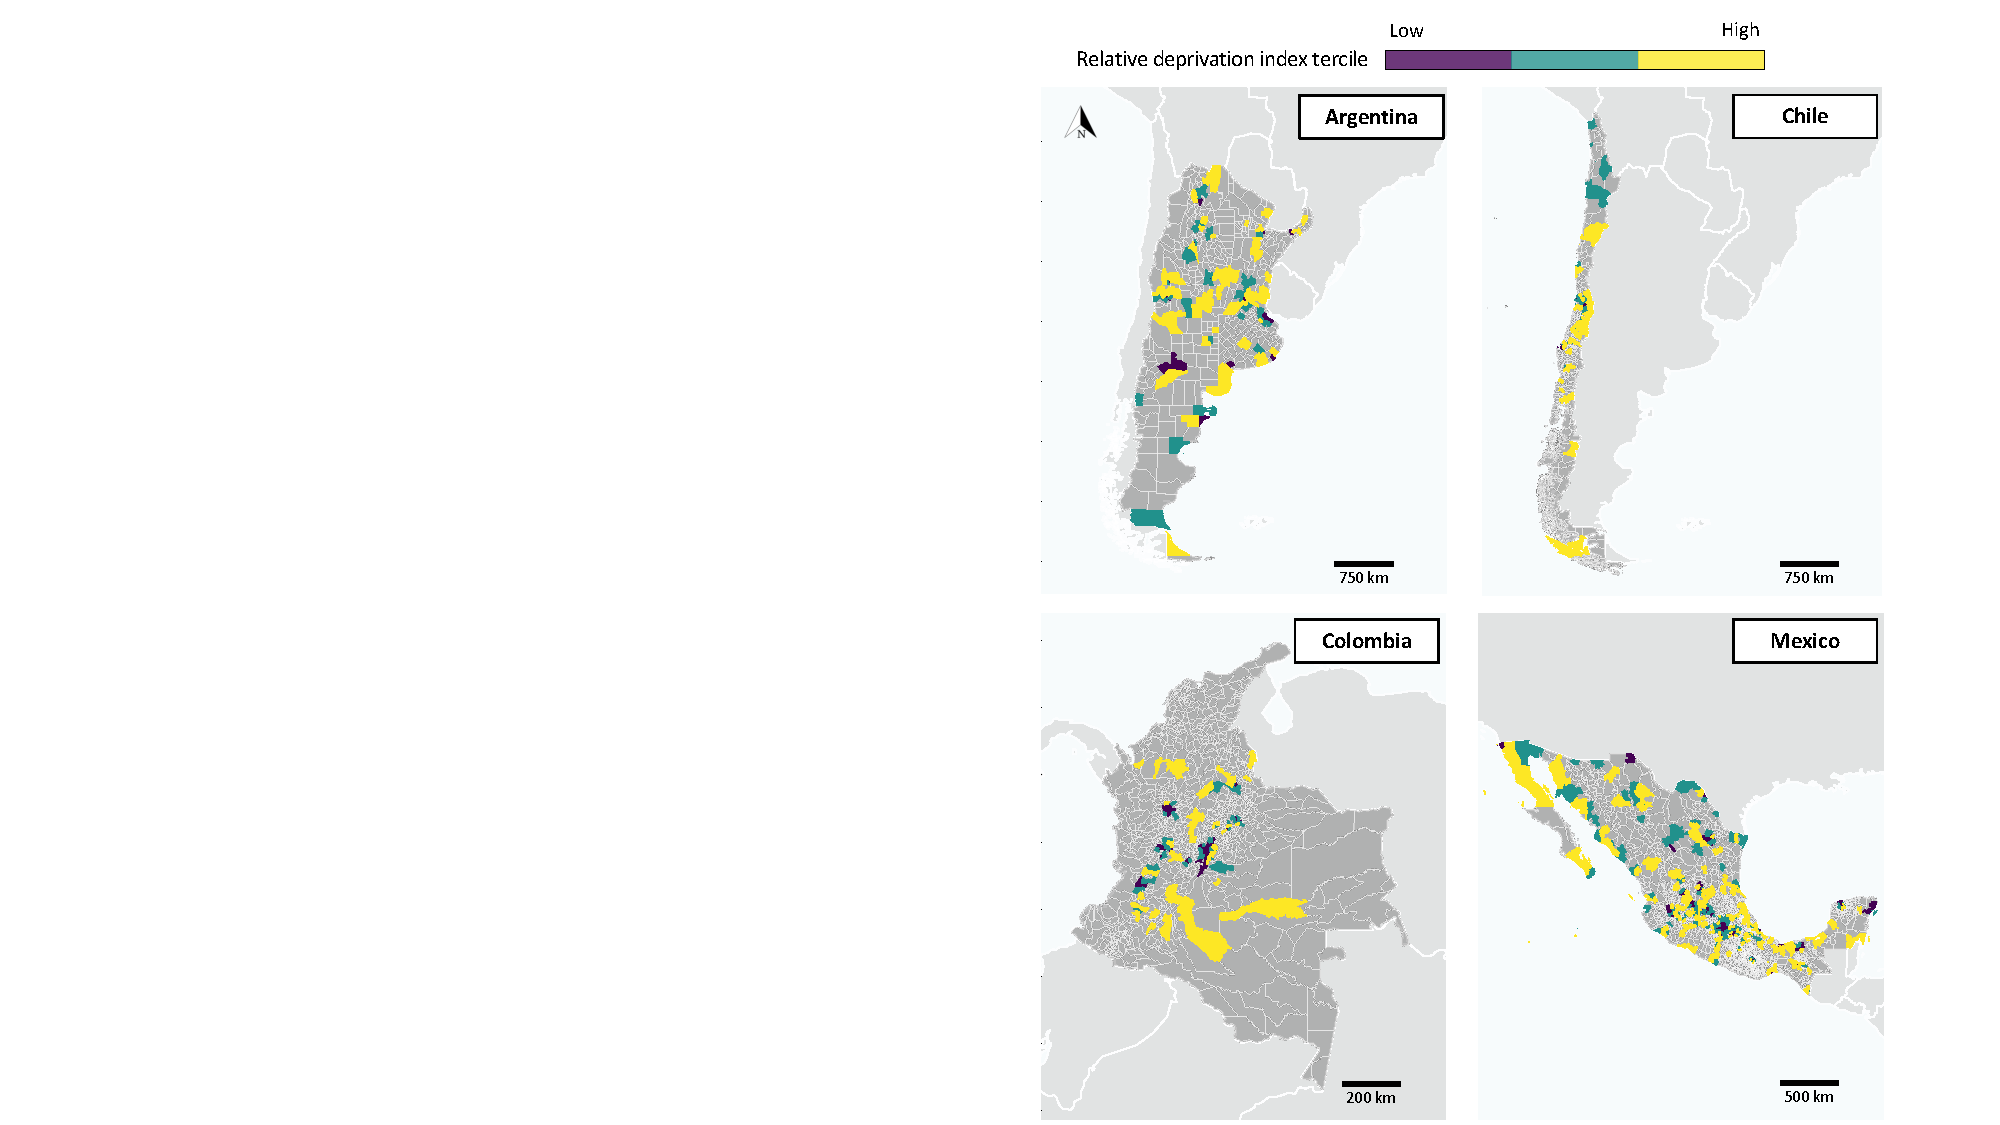
\includegraphics{figures/maps.pdf}

}

\caption{Administrative units within functional urban areas in
Argentina, Chile, Colombia and Mexico, coloured according to the average
Relative Deprivation Index.}

\end{figure}%

\subsection{The heterogeneous impact of COVID-19 on urban
mobility}\label{the-heterogeneous-impact-of-covid-19-on-urban-mobility}

We analyse the evolution of the percentage change in the number of
movements with respect to a baseline period prior to the pandemic.
Specifically, we focus the analysis on short-distance movements in urban
areas to represent local and routine mobility\textsuperscript{38}, so
only movements covering a distance of at most 70 km are considered. For
a movement to be classified as urban it needs to start or end within a
functional urban area from Argentina, Chile, Colombia and Mexico. The
observed data is available for a two-year period starting in April 2020,
just after the first wave of COVID-19 pandemic cases, and ending in
March 2022. After 2022 no observations are available, however, we
generate a 12-month forecast up to March 2023 in order to gain a better
understanding of the recovery trends.

Figure 2 displays the patterns of recovery for the mobility levels in
the administrative units belonging to functional urban areas in the
countries of interest. The three lines in each panel represent the mean
levels of mobility for administrative units grouped into one of three
terciles, according to their average RDI.

\begin{figure}[H]

{\centering \includegraphics{figures/prediction-rdi-band.pdf}

}

\caption{Patterns of recovery for urban mobility in administrative units
from Argentina, Chile, Colombia and Mexico.}

\end{figure}%

Generally, there was a drop in the levels of mobility with respect to
the baseline period in all four countries. This drop was especially
large for Argentina, Chile and Colombia, with Mexico displaying a
smaller decrease in the percentage change in the number of movements
with respect to the baseline. Following the initial drop in mobility,
all four countries evolve towards the recovery of baseline levels of
mobility, with a generally increasing trend. There are, however,
fluctuations from the general trend which manifest differently for each
country. These fluctuations mirror each other in the case of Argentina
and Colombia, where urban mobility sharply bounces back closer to
pre-pandemic levels around July of 2020. Chile and Mexico display more
progressive patterns of recovery, although Chile never reaches baseline
levels. These fluctuations are unique to each country and can be
attributed to local factors such as the effects of seasonality or the
different stringency measures imposed by the national governments during
the pandemic.

From Figure 2, we observe that there is a consistent tendency in how
administrative units with varying levels of deprivation were affected by
the pandemic. For all four countries, we observe that the administrative
units in the most deprived tercile are the ones that experienced the
smallest loss in levels of mobility at the beginning of the pandemic.
Differences in the levels of mobility across relative deprivation
terciles diminish with time. Argentina and Chile stand out as the
countries with the largest differences in mobility levels for different
relative deprivation terciles.

\subsection{The most deprived areas experienced the smallest drop in
mobility relative to pre-pandemic
levels}\label{the-most-deprived-areas-experienced-the-smallest-drop-in-mobility-relative-to-pre-pandemic-levels}

In this section we explore further the role of socioeconomic deprivation
in the evolution of the levels of urban mobility. For a given point in
time (i.e.~a month), we start by considering the relationship between
the percentage change in the number of movements relative to the
pre-pandemic baseline period and the average RDI, at the administrative
unit level. We assume that this relationship is linear and we use a
linear regression to estimate the slope and intercept characterising the
line of best fit. This is shown for April 2020 and March 2022 in the
right-hand side panels of Figure 3. After obtaining the slope and
intercept for every month, we are able to plot the evolution of these
parameters for both the observed and forecasted data, as displayed on
the left-hand-side panels of the same Figure.

\begin{figure}[H]

{\centering \includegraphics{figures/regression-evo-nobackground.pdf}

}

\caption{Evolution of the parameters characterising the relationship
between relative deprivation index and the percentage change in the
number of movements relative to the pre-pandemic baseline level of
mobility.}

\end{figure}%

We find patterns in the evolution of the estimated parameters that
characterise the relationship between the levels of urban mobility and
RDI. In Argentina, Colombia and Mexico, we observe that the slope of
this relationship evolves to become smaller over time. The tendency is
not apparent in Chile, where the slope of the relationship remains
approximately the same over time despite the temporary fluctuations. The
slope captures the extent of differences in the level of urban mobility
across administrative units with varying levels of socioeconomic
deprivation. It can therefore be regarded as a measure of inequality in
mobility patterns across socioeconomic groups. A slope equal to zero
would mean that all administrative units display the same level of
mobility regardless of their average RDI. Given the patterns observed in
Argentina, Colombia and Mexico, we find that at the beginning of the
pandemic there were notable inequalities between socioeconomic groups in
terms of the levels of urban mobility. While it has taken more than two
years for Argentina and Mexico to close the gap (their slope is close to
zero from spring 2022), inequalities persist in Chile and Colombia as of
March 2023.

The intercept of the relationship displays stronger patterns, which are
consistent across the four countries. The intercept estimates the urban
mobility levels that would be observed in administrative units where the
RDI is zero. The intercept was below the baseline level at the early
stages of the pandemic. As observed in Figure 3, while there are some
differences between countries in the evolution of the intercept, the
general tendency is for the intercept to increase. While Argentina and
Mexico reach values that are closer to the baseline towards the end of
the forecast period, the intercept for Chile and Colombia remains lower.
Therefore, if there were areas with no socioeconomic deprivation, we
would have seen a recovery in the levels of mobility, especially in
Argentina and Mexico

\section{Discussion}\label{sec-discussion}

Using location data from Meta-Facebook users, our study aimed to examine
the evolution of patterns of mobility across socioeconomic groups in
functional urban areas from Argentina, Chile, Colombia and Mexico from
April 2020 to March 2023, following the COVID-19 pandemic. We found a
systematic drop in the number of population movements in April 2020,
with the largest reductions observed in the most affluent administrative
units within functional urban areas (FUAs) from Argentina, Chile and
Colombia. While mobility rebounded closer to pre-pandemic levels
approximately two years later, when COVID-19 restrictions eased, the
number of movements remained below pre-pandemic in Chile. Furthermore,
we found that at the beginning of the pandemic there were inequalities
between socioeconomic groups in terms of the levels of urban mobility.
While it has taken more than two years for Argentina and Mexico to
gradually reduce gap, inequalities persist as of March 2023, especially
in Chile and Colombia according to our estimated data.

We focused the analysis on short-distance movements in urban areas,
especifically those covering 70 km or less. These journeys are typically
considered to represent local and routine mobility\textsuperscript{38} .
However, due to the characteristics of the Meta-Facebook movement data,
we are unable to distinguish the purpose of these short-distance
movements. Hence, some of our data could be capturing journeys that
involve a permanent change of place of residence. Our work therefore
motivates the need to answer questions regarding the validity of digital
footprint data for the analysis of human mobility. Further research
should focus on inferring more specific information about the nature of
the journeys, following similar approaches to those proposed
by\textsuperscript{42}, and quantifying the extent to which the digital
footprint data mirrors the true mobility patterns.

Conducting research on urban mobility using digital footprint data is
not straightforward, due to the challenges in accessing and working with
unstructured data sets which are often subject to biases and statistical
representation issues. These biases often arise from inequalities in
access and usage of digital technologies across demographic
groups\textsuperscript{43}. Despite these challenges, the data and
analysis that we used for this work provide evidence for non-trivial
patterns that are consistent across four countries in Latin America and
with other parts of the world. Our findings highlight the dynamic
interplay between socioeconomic status and urban mobility, and shall be
used to motivate and inform the public debate regarding the deep
societal consequences of urban mobility disparities on the wider
socioeconomic landscape of Latin American countries.

In conclusion, we argue that this work goes beyond the analysis of
specific patterns by demonstrating the potential of digital footprint
data for policy-relevant research on human mobility at an unprecedented
level of spatiotemporal granularity. While we have seen a rise in
initiatives to improve data services and methodological frameworks to
facilitate the use of digital footprint data for social good, progress
is still limited, especially in some parts of the world including Latin
America. It is in the hands of governments and public organisations to
prioritise the maximisation the societal benefits that digital footprint
data has to offer. This includes engaging in activities such as building
strategic partnerships with commercial data-holders and academic
institutions to establish a unified framework for the use of digital
footprint data in policy and research. In particular, we call for the
creation of resources like those developed by the European Commission
Joint Research Centre\textsuperscript{44} and the UN Statistics
Division\textsuperscript{45}, which identify sources of non-traditional
data and set methodological protocols for incorporating mobile phone
data into official mobility statistics. While current resources tend to
have a global reach, we advocate for more tailored local initiatives
that acknowledge disparities in regional data availability and adoption
of digital technologies.

\section{Methods}\label{sec-methods}

\subsection{Meta-Facebook movement
data}\label{meta-facebook-movement-data}

To capture population movements, we used anonymised aggregate mobile
phone location data from Meta users for Argentina, Colombia, Chile and
Mexico, covering a 24-month period from April 2020 to March 2022. We
used the dataset Facebook Movements created by Meta and accessed through
their Data for Good Initiative (\url{https://dataforgood.facebook.com}).
The data are built from Facebook app users who have the location
services setting turned on on their smartphone. Prior to releasing the
datasets, Meta ensures privacy and anonymity by removing personal
information and applying privacy-preserving
techniques\textsuperscript{46}. Small-count dropping is one of these
techniques. A data entry is removed if the population or movement count
for an area is lower than 10. The removal of small counts may mean that
population counts in small sparsely populated areas are not captured. A
second technique consists in adding a small undisclosed amount of random
noise to ensure that it is not possible to ascertain precise, true
counts for sparsely populated locations. Third, spatial smoothing using
inverse distance-weighted averaging is also applied is applied to
produce a smooth population count surface. The Facebook Movements
dataset offers information on the total number of Facebook users moving
between and within spatial units in the form of origin-destination
matrices. The data is temporally aggregated into three daily 8-hour time
windows (i.e.~00:00-08:00, 08:00-16:00 and 16:00-00:00). The dataset
includes a baseline capturing the number of movements before COVID-19
based on a 45-day period ending on March 10th 2020. The baseline is
computed using an average for the same time of the day and day of the
week in the period preceding March 10th. For instance, the baseline for
Monday 00:00-08:00 time window is obtained by averaging over data
collected on Mondays from 00:00 to 8:00 for the 45-day period. Details
about the baseline can be found in\textsuperscript{46}. The Bing Maps
Tile System developed by Microsoft (Microsoft) is used a spatial
framework to organise the data. The Tile System is a geospatial indexing
system that partitions the world into tile cells in a hierarchical way,
comprising 23 different levels of detail (Microsoft). At the lowest
level of detail (Level 1), the world is divided into four tiles with a
coarse spatial resolution. At each successive level, the resolution
increases by a factor of two. The data that we used are spatially
aggregated into Bing tile levels 13. That is about 4.9 x 4.9km at the
Equator\textsuperscript{46}.

\subsection{Spatiotemporal data
aggregation}\label{spatiotemporal-data-aggregation}

Since the focus of this work is on urban mobility, we focus the analysis
on Functional Urban Areas (FUAs), defined by the Global Human Settlement
Layer (GHSL). The spatial extent of the FUAs is often large and may
include several towns and neighbourhoods displaying a variety of
socioeconomic characteristics, hence using FUAs as the spatial units of
aggregation would considerably mask the heterogeneity in the mobility
patterns. While the original unit of aggregation for the movement data,
i.e.~the tiles from the Bing Maps Tile System, offers the highest degree
of spatial granularity available, the interpretation of findings from an
analysis based on administrative units is often more valuable. For this
reason, we perform a spatial join to aggregate the movement data into
administrative units at the GADM level 2 or 3. Only flows of people
starting or ending within the boundaries of a FUA are considered.

While the original movement data is originally aggregated into 8-hour
windows, this resolution is too fine for our analysis. Since the
analysis is focused on the longer-term evolution of patterns of urban
mobility, we aggregate the movement data by month.

In our analysis, we use the Relative Deprivation Index (RDI) as a
measure of socioeocnomic deprivation. The RDI data is made available via
NASA's Socioeconomic Data and Applications Centre (SEDAC), with a
spatial resolution of 1km pixels. We perform a spatial join of the
gridded data and the administrative units and compute the average RDI
within each of these administrative units.

\subsection{Time series analysis}\label{time-series-analysis}

For the countries included in the analysis, the movement data is
available until March 2022. In order to gain a better understanding of
the recovery trends after the pandemic, we generate a 12-month forecast
up to March 2023. This is done using Prophet\textsuperscript{27}, a
procedure developed by Meta's Core Data Science team to forecast time
series data based on an additive model. Prophet stands out from other
forecasting methods due to its ability to capture recurring seasonal
trends inherent in mobility data, such as fluctuations during holidays,
or changes in the general trend due to the impact of particular
circumstances, such as the COVID-19 pandemic. It is particularly
intuitive to use compared to other models due to its automated
trend-detection capabilities, making it accessible to users with no
expertise on the underlying model, while being robust to missing data
and outliers. For the analysis in this paper, yearly seasonality effects
are included as they yield the most realistic predictions.

Figures 2 and 3 have been created by removing statistical outliers. We
define these as the administrative units which, at any given month, have
a z-score greater than 4 for the percentage change in the number of
movements. Furthermore, a Savitzky-Golay filter is applied to smooth the
time series data, using a length of 4 units for the filter window and
order 2 polynomials to fit the samples.

\section*{References}\label{references}
\addcontentsline{toc}{section}{References}

\phantomsection\label{refs}
\begin{CSLReferences}{0}{0}
\bibitem[\citeproctext]{ref-ackers2005}
\CSLLeftMargin{1. }%
\CSLRightInline{Ackers, L.
\href{https://doi.org/10.1111/j.1468-2435.2005.00343.x}{Moving People
and Knowledge: Scientific Mobility in the European Union1}.
\emph{International Migration} \textbf{43}, 99--131 (2005).}

\bibitem[\citeproctext]{ref-chen2016}
\CSLLeftMargin{2. }%
\CSLRightInline{Chen, C., Ma, J., Susilo, Y., Liu, Y. \& Wang, M.
\href{https://doi.org/10.1016/j.trc.2016.04.005}{The promises of big
data and small data for travel behavior (aka human mobility) analysis}.
\emph{Transportation Research Part C: Emerging Technologies}
\textbf{68}, 285--299 (2016).}

\bibitem[\citeproctext]{ref-belik2011}
\CSLLeftMargin{3. }%
\CSLRightInline{Belik, V., Geisel, T. \& Brockmann, D.
\href{https://doi.org/10.1103/physrevx.1.011001}{Natural Human Mobility
Patterns and Spatial Spread of Infectious Diseases}. \emph{Physical
Review X} \textbf{1}, (2011).}

\bibitem[\citeproctext]{ref-klugman2009human}
\CSLLeftMargin{4. }%
\CSLRightInline{Klugman, J. Human development report 2009. Overcoming
barriers: Human mobility and development. \emph{Overcoming Barriers:
Human Mobility and Development (October 5, 2009). UNDP-HDRO Human
Development Reports} (2009).}

\bibitem[\citeproctext]{ref-barbosa2018}
\CSLLeftMargin{5. }%
\CSLRightInline{Barbosa, H. \emph{et al.}
\href{https://doi.org/10.1016/j.physrep.2018.01.001}{Human mobility:
Models and applications}. \emph{Physics Reports} \textbf{734}, 1--74
(2018).}

\bibitem[\citeproctext]{ref-chinazzi2020}
\CSLLeftMargin{6. }%
\CSLRightInline{Chinazzi, M. \emph{et al.}
\href{https://doi.org/10.1126/science.aba9757}{The effect of travel
restrictions on the spread of the 2019 novel coronavirus (COVID-19)
outbreak}. \emph{Science} \textbf{368}, 395--400 (2020).}

\bibitem[\citeproctext]{ref-nouvellet2021}
\CSLLeftMargin{7. }%
\CSLRightInline{Nouvellet, P. \emph{et al.}
\href{https://doi.org/10.1038/s41467-021-21358-2}{Reduction in mobility
and COVID-19 transmission}. \emph{Nature Communications} \textbf{12},
(2021).}

\bibitem[\citeproctext]{ref-rowe2023}
\CSLLeftMargin{8. }%
\CSLRightInline{Rowe, F., González-Leonardo, M. \& Champion, T. Virtual
special issue: Internal migration in times of COVID{-}19.
\emph{Population, Space and Place} (2023)
doi:\href{https://doi.org/10.1002/psp.2652}{10.1002/psp.2652}.}

\bibitem[\citeproctext]{ref-abdullah2020}
\CSLLeftMargin{9. }%
\CSLRightInline{Abdullah, M., Dias, C., Muley, D. \& Shahin, Md.
\href{https://doi.org/10.1016/j.trip.2020.100255}{Exploring the impacts
of COVID-19 on travel behavior and mode preferences}.
\emph{Transportation Research Interdisciplinary Perspectives}
\textbf{8}, 100255 (2020).}

\bibitem[\citeproctext]{ref-bonaccorsi2020}
\CSLLeftMargin{10. }%
\CSLRightInline{Bonaccorsi, G. \emph{et al.}
\href{https://doi.org/10.1073/pnas.2007658117}{Economic and social
consequences of human mobility restrictions under COVID-19}.
\emph{Proceedings of the National Academy of Sciences} \textbf{117},
15530--15535 (2020).}

\bibitem[\citeproctext]{ref-abu-rayash2020}
\CSLLeftMargin{11. }%
\CSLRightInline{Abu-Rayash, A. \& Dincer, I.
\href{https://doi.org/10.1016/j.erss.2020.101693}{Analysis of mobility
trends during the COVID-19 coronavirus pandemic: Exploring the impacts
on global aviation and travel in selected cities}. \emph{Energy Research
\& Social Science} \textbf{68}, 101693 (2020).}

\bibitem[\citeproctext]{ref-lee2023}
\CSLLeftMargin{12. }%
\CSLRightInline{Lee, S., Ko, E., Jang, K. \& Kim, S.
\href{https://doi.org/10.1016/j.cities.2023.104223}{Understanding
individual-level travel behavior changes due to COVID-19: Trip
frequency, trip regularity, and trip distance}. \emph{Cities}
\textbf{135}, 104223 (2023).}

\bibitem[\citeproctext]{ref-borkowski2021}
\CSLLeftMargin{13. }%
\CSLRightInline{Borkowski, P., Jażdżewska-Gutta, M. \& Szmelter-Jarosz,
A. \href{https://doi.org/10.1016/j.jtrangeo.2020.102906}{Lockdowned:
Everyday mobility changes in response to COVID-19}. \emph{Journal of
Transport Geography} \textbf{90}, 102906 (2021).}

\bibitem[\citeproctext]{ref-chang2020}
\CSLLeftMargin{14. }%
\CSLRightInline{Chang, S. \emph{et al.}
\href{https://doi.org/10.1038/s41586-020-2923-3}{Mobility network models
of COVID-19 explain inequities and inform reopening}. \emph{Nature}
\textbf{589}, 82--87 (2020).}

\bibitem[\citeproctext]{ref-fraiberger2020}
\CSLLeftMargin{15. }%
\CSLRightInline{Fraiberger, S. P. \emph{et al.} Uncovering socioeconomic
gaps in mobility reduction during the COVID-19 pandemic using location
data. (2020)
doi:\href{https://doi.org/10.48550/ARXIV.2006.15195}{10.48550/ARXIV.2006.15195}.}

\bibitem[\citeproctext]{ref-weill2020}
\CSLLeftMargin{16. }%
\CSLRightInline{Weill, J. A., Stigler, M., Deschenes, O. \& Springborn,
M. R. \href{https://doi.org/10.1073/pnas.2009412117}{Social distancing
responses to COVID-19 emergency declarations strongly differentiated by
income}. \emph{Proceedings of the National Academy of Sciences}
\textbf{117}, 19658--19660 (2020).}

\bibitem[\citeproctext]{ref-dueuxf1as2021}
\CSLLeftMargin{17. }%
\CSLRightInline{Dueñas, M., Campi, M. \& Olmos, L. E.
\href{https://doi.org/10.1057/s41599-021-00775-0}{Changes in mobility
and socioeconomic conditions during the COVID-19 outbreak}.
\emph{Humanities and Social Sciences Communications} \textbf{8},
(2021).}

\bibitem[\citeproctext]{ref-santana2023}
\CSLLeftMargin{18. }%
\CSLRightInline{Santana, C. \emph{et al.} COVID-19 is linked to changes
in the time{\textendash}space dimension of human mobility. \emph{Nature
Human Behaviour} (2023)
doi:\href{https://doi.org/10.1038/s41562-023-01660-3}{10.1038/s41562-023-01660-3}.}

\bibitem[\citeproctext]{ref-florida2021}
\CSLLeftMargin{19. }%
\CSLRightInline{Florida, R., Rodríguez-Pose, A. \& Storper, M.
\href{https://doi.org/10.1177/00420980211018072}{Critical Commentary:
Cities in a post-COVID world}. \emph{Urban Studies} \textbf{60},
1509--1531 (2021).}

\bibitem[\citeproctext]{ref-rowe2023a}
\CSLLeftMargin{20. }%
\CSLRightInline{Rowe, F., Cabrera-Arnau, C., González-Leonardo, M.,
Nasuto, A. \& Neville, R. Reduced mobility? Urban exodus? Medium-term
impacts of the COVID-19 pandemic on internal population movements in
latin american countries. (2023)
doi:\href{https://doi.org/10.48550/ARXIV.2311.01464}{10.48550/ARXIV.2311.01464}.}

\bibitem[\citeproctext]{ref-barrero2021}
\CSLLeftMargin{21. }%
\CSLRightInline{Barrero, J. M., Bloom, N. \& Davis, S. \emph{Why working
from home will stick}. \url{http://dx.doi.org/10.3386/w28731} (2021)
doi:\href{https://doi.org/10.3386/w28731}{10.3386/w28731}.}

\bibitem[\citeproctext]{ref-aksoy2022}
\CSLLeftMargin{22. }%
\CSLRightInline{Aksoy, C. G. \emph{et al.} \emph{Working from home
around the world}. \url{http://dx.doi.org/10.3386/w30446} (2022)
doi:\href{https://doi.org/10.3386/w30446}{10.3386/w30446}.}

\bibitem[\citeproctext]{ref-green2021}
\CSLLeftMargin{23. }%
\CSLRightInline{Green, M., Pollock, F. D. \& Rowe, F. New forms of data
and new forms of opportunities to monitor and tackle a pandemic. in
423--429 (Springer International Publishing, 2021).
doi:\href{https://doi.org/10.1007/978-3-030-70179-6_56}{10.1007/978-3-030-70179-6\_56}.}

\bibitem[\citeproctext]{ref-bell2014}
\CSLLeftMargin{24. }%
\CSLRightInline{Bell, M. \emph{et al.}
\href{https://doi.org/10.1002/psp.1848}{Internal Migration Data Around
the World: Assessing Contemporary Practice}. \emph{Population, Space and
Place} \textbf{21}, 1--17 (2014).}

\bibitem[\citeproctext]{ref-rowe2023big}
\CSLLeftMargin{25. }%
\CSLRightInline{Rowe, F. Big data. in \emph{Concise encyclopedia of
human geography} 42--47 (Edward Elgar Publishing, 2023).}

\bibitem[\citeproctext]{ref-calafiore2023}
\CSLLeftMargin{26. }%
\CSLRightInline{Calafiore, A., Samardzhiev, K., Rowe, F., Fleischmann,
M. \& Arribas-Bel, D. Inequalities in experiencing urban functions. An
exploration of human digital (geo-)footprints. \emph{Environment and
Planning B: Urban Analytics and City Science} (2023)
doi:\href{https://doi.org/10.1177/23998083231208507}{10.1177/23998083231208507}.}

\bibitem[\citeproctext]{ref-prophet17}
\CSLLeftMargin{27. }%
\CSLRightInline{Taylor, S. J. \& Letham, B.
\href{https://doi.org/10.7287/peerj.preprints.3190v2}{Forecasting at
scale}. \emph{PeerJ Preprints} \textbf{5}, e3190v2 (2017).}

\bibitem[\citeproctext]{ref-GHSL19}
\CSLLeftMargin{28. }%
\CSLRightInline{Schiavina M., M. L., Moreno-Monroy A. GHS-FUA R2019A -
GHS functional urban areas, derived from GHS-UCDB R2019A, (2015),
R2019A. (2019).}

\bibitem[\citeproctext]{ref-RDI2022}
\CSLLeftMargin{29. }%
\CSLRightInline{Columbia University, C. for I. E. S. I. Network. C.
Global gridded relative deprivation index (GRDI), version 1. (2022)
doi:\href{https://doi.org/10.7927/3xxe-ap97}{10.7927/3xxe-ap97}.}

\bibitem[\citeproctext]{ref-roweCalafiore2022}
\CSLLeftMargin{30. }%
\CSLRightInline{Rowe, F., Calafiore, A., Arribas-Bel, D., Samardzhiev,
K. \& Fleischmann, M. Urban exodus? Understanding human mobility in
britain during the COVID-19 pandemic using facebook data. (2022)
doi:\href{https://doi.org/10.48550/ARXIV.2206.03272}{10.48550/ARXIV.2206.03272}.}

\bibitem[\citeproctext]{ref-wang2022}
\CSLLeftMargin{31. }%
\CSLRightInline{Wang, Y., Zhong, C., Gao, Q. \& Cabrera-Arnau, C.
\href{https://doi.org/10.1007/s44212-022-00018-w}{Understanding internal
migration in the UK before and during the COVID-19 pandemic using
twitter data}. \emph{Urban Informatics} \textbf{1}, (2022).}

\bibitem[\citeproctext]{ref-de2004inequality}
\CSLLeftMargin{32. }%
\CSLRightInline{De Ferranti, D. M. \emph{Inequality in latin america:
Breaking with history?} (World Bank publications, 2004).}

\bibitem[\citeproctext]{ref-carranza2023wealth}
\CSLLeftMargin{33. }%
\CSLRightInline{Carranza, R., De Rosa, M. \& Flores, I. Wealth
inequality in latin america. (2023).}

\bibitem[\citeproctext]{ref-united2023world}
\CSLLeftMargin{34. }%
\CSLRightInline{United Nations, D. for E. \& Affairs., S. \emph{World
population prospects 2022: Summary of results}. (UN, 2023).}

\bibitem[\citeproctext]{ref-milanovic2016global}
\CSLLeftMargin{35. }%
\CSLRightInline{Milanovic, B. \emph{Global inequality: A new approach
for the age of globalization}. (Harvard University Press, 2016).}

\bibitem[\citeproctext]{ref-habitat2022world}
\CSLLeftMargin{36. }%
\CSLRightInline{Habitat, U. World cities report 2022: Envisaging the
future of cities. \emph{United Nations Human Settlements Programme:
Nairobi, Kenya} 41--44 (2022).}

\bibitem[\citeproctext]{ref-GADM24}
\CSLLeftMargin{37. }%
\CSLRightInline{GADM. GADM maps and data. (2024).}

\bibitem[\citeproctext]{ref-owen1992migration}
\CSLLeftMargin{38. }%
\CSLRightInline{Owen, D. \& Green, A. Migration patterns and trends. in
\emph{Migration processes and patterns: Research progress and prospects}
(eds. Champion, T. \& Fielding, T.) (Belhaven Press, 1992).}

\bibitem[\citeproctext]{ref-LaurenAlexander15}
\CSLLeftMargin{39. }%
\CSLRightInline{Alexander, L., Jiang, S., Murga, M. \& González, M. C.
\href{https://doi.org/10.1016/j.trc.2015.02.018}{Origin--destination
trips by purpose and time of day inferred from mobile phone data}.
\emph{Transportation Research Part C: Emerging Technologies}
\textbf{58}, 240--250 (2015).}

\bibitem[\citeproctext]{ref-MengChuishi17}
\CSLLeftMargin{40. }%
\CSLRightInline{Meng, C., Cui, Y., He, Q., Su, L. \& Gao, J. Travel
purpose inference with GPS trajectories, POIs, and geo-tagged social
media data. in \emph{2017 IEEE international conference on big data (big
data)} 1319--1324 (2017).
doi:\href{https://doi.org/10.1109/BigData.2017.8258062}{10.1109/BigData.2017.8258062}.}

\bibitem[\citeproctext]{ref-NiluferSariAslam21}
\CSLLeftMargin{41. }%
\CSLRightInline{Nilufer Sari Aslam, T. C., Mohamed R. Ibrahim \& Zhang,
Y. \href{https://doi.org/10.1080/10095020.2021.1985943}{ActivityNET:
Neural networks to predict public transport trip purposes from
individual smart card data and POIs}. \emph{Geo-spatial Information
Science} \textbf{24}, 711--721 (2021).}

\bibitem[\citeproctext]{ref-Cabrera-Arnau2023}
\CSLLeftMargin{42. }%
\CSLRightInline{Cabrera-Arnau, C., Zhong, C., Batty, M., Silva, R. \&
Kang, S. M. \href{https://doi.org/10.1038/s41598-023-33003-7}{Inferring
urban polycentricity from the variability in human mobility patterns}.
\emph{Scientific Reports} \textbf{13}, 5751 (2023).}

\bibitem[\citeproctext]{ref-RoweBigData23}
\CSLLeftMargin{43. }%
\CSLRightInline{Rowe, F. 9.: Big data. in \emph{Concise encyclopedia of
human geography} 42--47 (Edward Elgar Publishing, 2023).
doi:\href{https://doi.org/10.4337/9781800883499.ch09}{10.4337/9781800883499.ch09}.}

\bibitem[\citeproctext]{ref-ECJRC22}
\CSLLeftMargin{44. }%
\CSLRightInline{Commission, E. \emph{et al.} \emph{Data innovation in
demography, migration and human mobility}. (Publications Office of the
European Union, 2022).
doi:\href{https://doi.org/doi/10.2760/027157}{doi/10.2760/027157}.}

\bibitem[\citeproctext]{ref-UNSD}
\CSLLeftMargin{45. }%
\CSLRightInline{Division, U. N. S. Handbook on the use of mobile phone
data for official statistics. (2019).}

\bibitem[\citeproctext]{ref-Maas19}
\CSLLeftMargin{46. }%
\CSLRightInline{Maas, P. \emph{et al.} Facebook disaster maps: Aggregate
insights for crisis response and recovery. in \emph{16th international
conference on information systems for crisis response and management}
836--847 (2019).}

\end{CSLReferences}



\end{document}
